\section{Discussion}
\label{cha:discussion}
This research aims to establish a predictive framework for application benchmark performance based on microbenchmark execution results. The study ensures that both benchmarking types are conducted in controlled yet realistic environments. The discussion below summarizes key insights acknowledges limitations and suggests further work that other researchers can do. 

\subsection{Application benchmarks and Microbenchmarks}
The application benchmark experiments, executed over five pairs of versions shown in  \cref{tab:compared_versions}—v1.104-v1.105, v1.105-v1.106, v1.106-v1.107, v1.107-v1.108, and v1.108-v1.109 revealed consistent performance trends under load. The two-phased approach, consisting of data insertion followed by query execution, provided a comprehensive view of the \ac{SUT}'s behavior and how it evolved between versions. \cref{fig:mean_inserts_time_all_runs-v104-v105,fig:mean_inserts_time_all_runs-v105-v106,fig:mean_inserts_time_all_runs-v106-v107,fig:mean_inserts_time_all_runs-v107-v108,fig:mean_inserts_time_all_runs-v108-v109,fig:mean_inserts_time_all_runs-v107-v108,fig:mean_query_rate_all_runs-v104-v105,fig:mean_query_rate_all_runs-v105-v106,fig:mean_query_rate_all_runs-v106-v107,fig:mean_query_rate_all_runs-v107-v108,fig:mean_query_rate_all_runs-v108-v109} clearly showed that, regardless of the model's limitations, performance changes across versions were evident in the graphs. \cref{fig:insertTime,fig:mean_query_rate} show that code changes lead to performance improvements or regressions, even when the current predictive model does not fully capture the underlying relationship and cannot adequately represent its link. \\
During the application benchmarks' execution, we identified several resource allocation challenges, particularly related to the \ac{SUT}'s we configured the virtual machines provisioned for the benchmark using the e2-standard-2 allocation of resources; however, during the data insertion phase, the \ac{SUT} encountered connection reset errors, which ended the insertion process and invalidated the run of the group-by queries. We no longer faced the error after increasing the memory and \ac{CPU} available to the docker containers while keeping the \ac{SUT} under heavy resource usage.\\
The adjustment required for memory and \ac{CPU} availability underlines an important distinction between application benchmarks and microbenchmarks. Since microbenchmarks measure the performance of specific functions, while application benchmarks measure the performance of the whole application, significantly more resources are required to simulate real-world workloads accurately. These additional resources, given to the application benchmark, led to a challenge when comparing performance measurements across benchmarking techniques as they created a difference in the setup of both benchmarks. However, as application benchmarks are supposed to require larger resource allocation than microbenchmarks to manage and provide realistic operating workloads, this research believes that this was expected and does not invalidate the results because application benchmarks operate in environments where resource constraints, I/O bottlenecks and concurrency effects impact performance. \\ 
On the other hand, even though microbenchmarks are easier to set up compared to application benchmarks as they focus solely on individual functions, this research finds that they took, on average, 8 hours to run, as shown in \cref{tab:version_time}. We expected the experiments to take longer due to the techniques applied when running the microbenchmarks. However, this will challenge including the microbenchmarks in \ac{CI}/\ac{CD} pipelines because, on the one hand, the microbenchmarks require enough repetitions to provide accurate results, and on the other hand, waiting 8 hours for the pipeline to finish is not feasible. Therefore, their applicability to broader system performance is limited despite being executed hundreds of times for reliability. Additionally, high collinearity and redundancy among several microbenchmarks make it difficult to directly link micro-level performance changes to application-level outcomes. Thus, a performance optimization that appears effective in a microbenchmark function may lead to different results in an application benchmark. Given these findings, further work must be done with essential care to manage resource allocation in future performance evaluations to maintain accuracy and ensure benchmarking outcomes remain valid and comparable across various test environments. \\
Another challenge faced when running the microbenchmarks was the tool \ac{GoAbs} used to measure the microbenchmarks. This research also presented issues with the tool used to run microbenchmarks because, as stated before, this tool was modified by Grambow et al. \cite{grambow} and there was no clear documentation on how to be able to compare a pair of \ac{SUT}. This research fully relies on the modification made and only evaluates correctly the microbenchmarks that are common to both pairs of versions that are being tested.

\subsection{Challenges in Predicting Performance with Ridge Regression}
We use ridge regression to predict application benchmark performance based on microbenchmark results. This research uses Ridge regression due to its ability to handle collinearity through L2 regularization, which reduces the impact of highly correlated features \cite{mcdonald2009ridgeregression}. This research used one of the most common methods to measure errors when performing regressions: the Mean Square Error (\ac{MSE}) \cite{wang2009meansquareerror} and R-squared \cite{chicco2021coefficientofdetermination} as main metrics to be able to determine if their model was performing well or poorly. Furthermore, to select the best set of features possible for the model, we performed a collinearity analysis between the features to reduce the complexity of the model and have better results. In order to perform this analysis, we attempt to use two known methods; the first one is Principal Component Analysis, further referred to as Principal Component Analysis \ac{PCA} \cite{Jolliffe2002PCA}, and the Variance Inflation Factor, further referred to as Variance Inflation Factor \ac{VIF} \cite{thompson2017extractingVIF}. Despite our efforts, none of the mentioned methods yielded good results for the model. We will start by analyzing the efforts taken to perform \ac{PCA}, and then we will move to analyze \ac{VIF}.  \\ 
Jolliffe \cite{Jolliffe2002PCA} states that \ac{PCA} selects components to explain the most variation possible from the original variables in the features of microbenchmarks. However, this does not guarantee that the selected components will be the best for regression prediction. More importantly, another known limitation of \ac{PCA} is that this method assumes a linear transformation of the data \cite{Jolliffe2002PCA}, which is not the case in our research, as shown in \cref{cha:evaluation}. These two limitations of \ac{PCA} and the collinearity of the features did not allow for a dimensional reduction to select the best features possible to use in ridge regression. Some options can be applied to overcome the limitations of \ac{PCA}. Schölkopf et al. \cite{scholkopf1998nonlinearcomponent} state that a Kernel \ac{PCA} can address nonlinear data by mapping the features into a higher-dimensional space and then applying \ac{PCA}. However, due to a lack of expertise in advanced dimensionality reduction techniques, this research did not attempt to address these limitations. \\
The second method we attempted to use was \ac{VIF}; after this research failed to use \ac{PCA} to perform the feature selection for the model, we moved to analyze the collinearity of the features. Although Ridge regression has an L2 regularization that penalizes the features for their collinearity, this regression method presents some limitations when features have high collinearity. Therefore, as suggested by Thompson et al. \cite{thompson2017extractingVIF}, to address the high collinearity between the features, we attempted to use \ac{VIF} to remove highly correlated features. However, given the distribution of the data seen in \cref{fig:distribution_BenchmarkMergeBlockStreamsFourSourcesWorstCase-2,fig:distribution_BenchmarkParseProtobufRequest_scopes_1_rows_100_attributes_5-2,fig:distribution_BenchmarkQueueThroughputConcurrent_block,fig:distribution_BenchmarkUnmarshalDeltaConstArray-2}, \ac{VIF} is too strict to be applied for feature selection, as after running \ac{VIF}, we notice that the number of features selected was zero. This makes sense because, as stated before, we discovered that the collinearity between the microbenchmarks is very high.  \\
Given the poor results obtained by \ac{PCA} and \ac{VIF}, we decided to do a collinearity matrix between the features and remove the ones that were above a threshold of \text{99\%}, ultimately giving us the best \ac{MSE} and R-squared metrics. \\
However, the low R-squared values and high (\ac{MSE}) results show that the model suffers from overfitting. Indicating that ridge regression struggled to generalize effectively, limiting its reliability in predicting real-world application performance using microbenchmark results. Lastly, as also shown in \cref{fig:distribution_BenchmarkMergeBlockStreamsFourSourcesWorstCase-2,fig:distribution_BenchmarkParseProtobufRequest_scopes_1_rows_100_attributes_5-2,fig:distribution_BenchmarkQueueThroughputConcurrent_block,fig:distribution_BenchmarkUnmarshalDeltaConstArray-2} some clusters of points seem to show a distribution that might be explained by a linear regression method; this research does not analyze the data further due to time limitations and lack of expertise on how to perform this adjustment.  \\
\begin{figure}[!htbp]
    \captionsetup[subfigure]{list=true}
    \centering
    % -- Row 1: two subfigures --
    \begin{subfigure}[b]{0.9\textwidth}
        \centering
        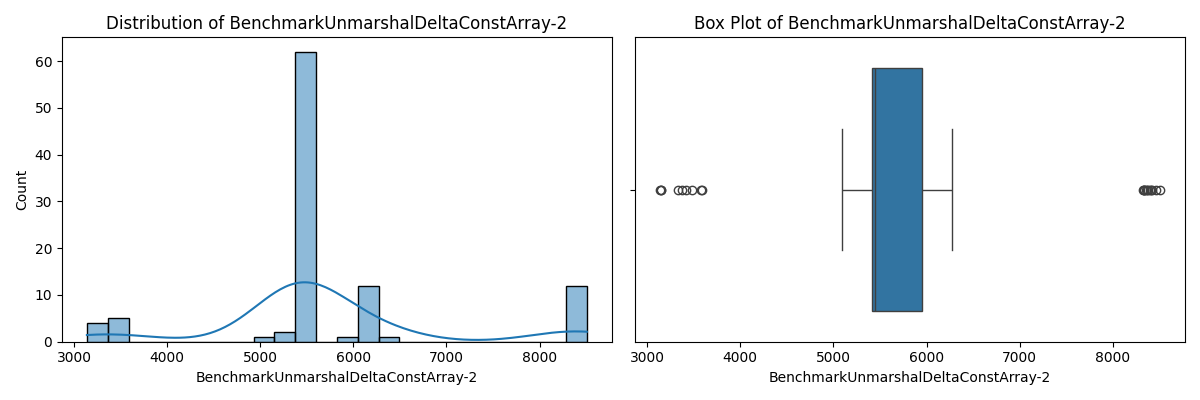
\includegraphics[width=\textwidth]{figures/distribution_BenchmarkUnmarshalDeltaConstArray-2.png}
        \caption{BenchmarkUnmarshalDeltaConstArray-2}
        \label{fig:distribution_BenchmarkUnmarshalDeltaConstArray-2}
    \end{subfigure}
      \vskip\baselineskip  % vertical space between rows
    \begin{subfigure}[b]{0.9\textwidth}
        \centering
        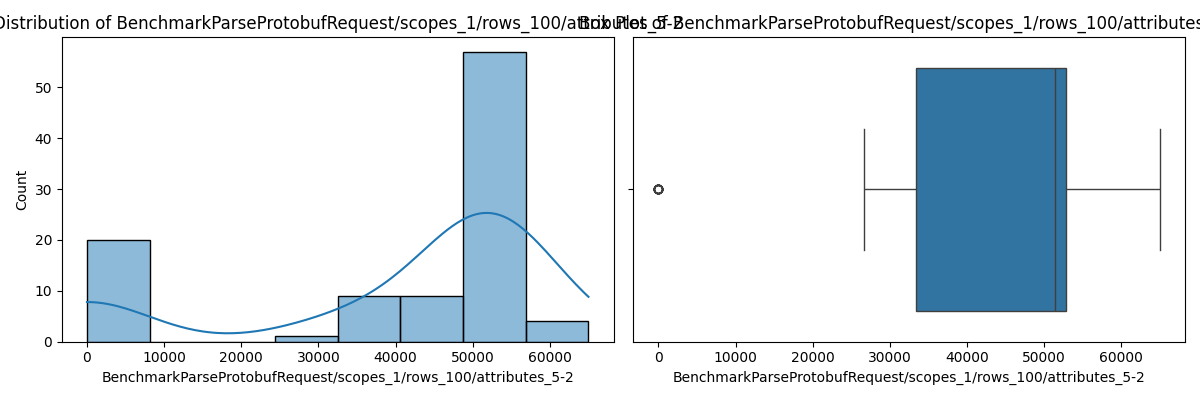
\includegraphics[width=\textwidth]{figures/distribution_BenchmarkParseProtobufRequest_scopes_1_rows_100_attributes_5-2.png}
        \caption{BenchmarkParseProtobufRequest-scopes-1-rows-100-attributes-5-2}
        \label{fig:distribution_BenchmarkParseProtobufRequest_scopes_1_rows_100_attributes_5-2}
    \end{subfigure}
          \vskip\baselineskip  % vertical space between rows
    \begin{subfigure}[b]{0.9\textwidth}
        \centering
        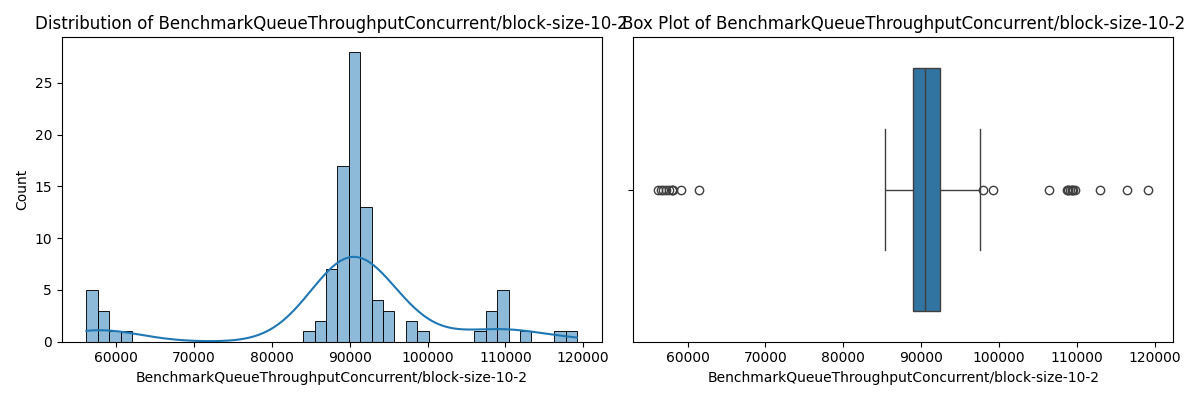
\includegraphics[width=\textwidth]{figures/distribution_BenchmarkQueueThroughputConcurrent_block-size-10-2.png}
        \caption{BenchmarkQueueThroughputConcurrent}
        \label{fig:distribution_BenchmarkQueueThroughputConcurrent_block}
    \end{subfigure}

    \vskip\baselineskip  % vertical space between rows
    \begin{subfigure}[b]{0.9\textwidth}
        \centering
        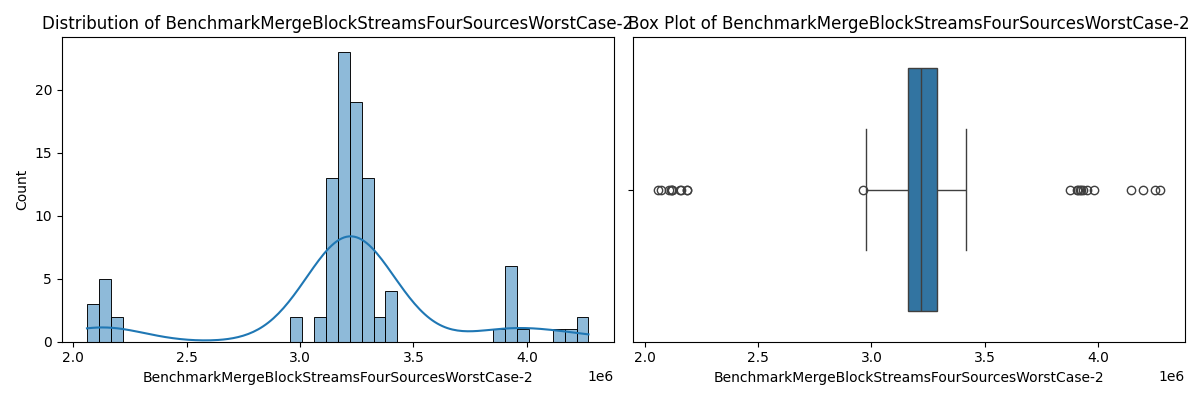
\includegraphics[width=\textwidth]{figures/distribution_BenchmarkMergeBlockStreamsFourSourcesWorstCase-2.png}
        \caption{BenchmarkMergeBlockStreamsFourSourcesWorstCase}
        \label{fig:distribution_BenchmarkMergeBlockStreamsFourSourcesWorstCase-2}
    \end{subfigure}
    \caption{Distribution Microbenchmarks}
    \label{fig:DistributionMicrobenchamrk}
\end{figure}
\cref{fig:distribution_BenchmarkUnmarshalDeltaConstArray-2,fig:distribution_BenchmarkParseProtobufRequest_scopes_1_rows_100_attributes_5-2,fig:distribution_BenchmarkMergeBlockStreamsFourSourcesWorstCase-2,fig:distribution_BenchmarkQueueThroughputConcurrent_block}
reveal distribution patterns that undermine our model. These do not follow a normal distribution presented across the benchmark functions. Instead, these figures present asymmetry, which prevents the ridge regression models from obtaining accurate results, instead presenting a high variance of the execution time leading to a fluctuating value across the experiment and a distribution where a significant number of observations have long tails toward higher execution times. These three key aspects explain why the ridge regression model fails to explain effectively and why alternative modeling techniques may be necessary to prove further the correlation between microbenchmarks and applications benchmarks performance.  

\begin{figure}[ht]
    \captionsetup[subfigure]{list=true}
    \centering
    \begin{subfigure}[b]{0.49\textwidth}
        \centering
        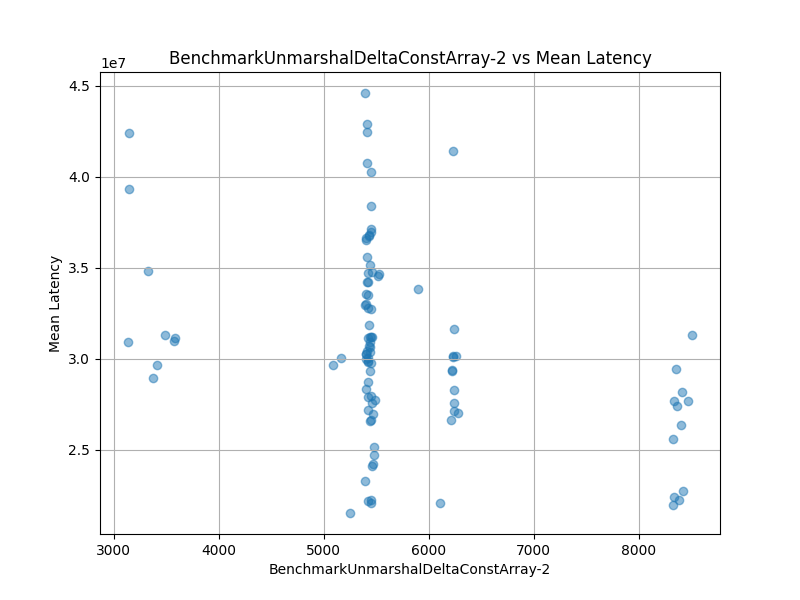
\includegraphics[width=\textwidth]{figures/BenchmarkUnmarshalDeltaConstArray-2_vs_mean_latency.png}
        \caption{BenchmarkUnmarshalDeltaConstArray vs mean query rate}
        \label{fig:BenchmarkUnmarshalDeltaConstArray-2_vs}
    \end{subfigure}
    \hfill
    \begin{subfigure}[b]{0.49\textwidth}
        \centering
        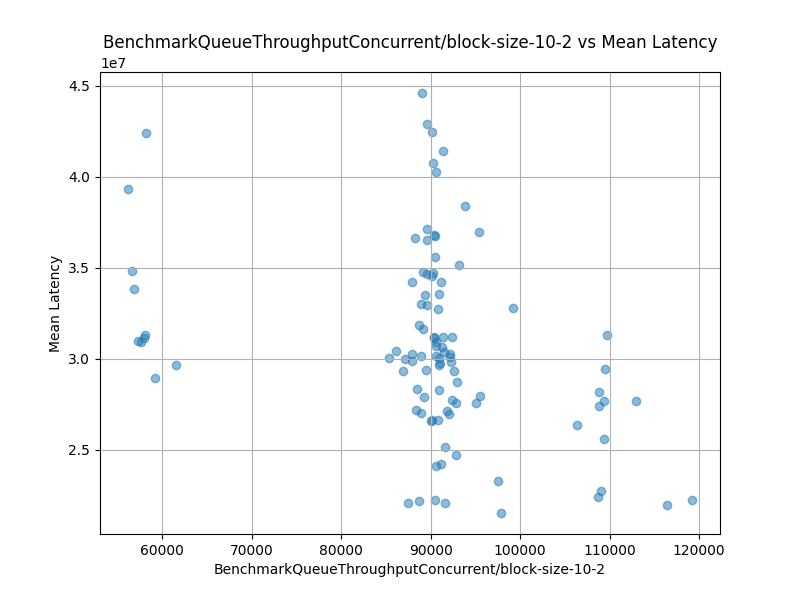
\includegraphics[width=\textwidth]{figures/BenchmarkQueueThroughputConcurrent_block-size-10-2_vs_mean_latency.png}
        \caption{BenchmarkQueueThroughputConcurrent vs mean query rate}
        \label{fig:BenchmarkQueueThroughputConcurrent_vs_mean_latency}
    \end{subfigure}

    \vskip\baselineskip  % vertical space between rows

    \begin{subfigure}[b]{0.45\textwidth}
        \centering
        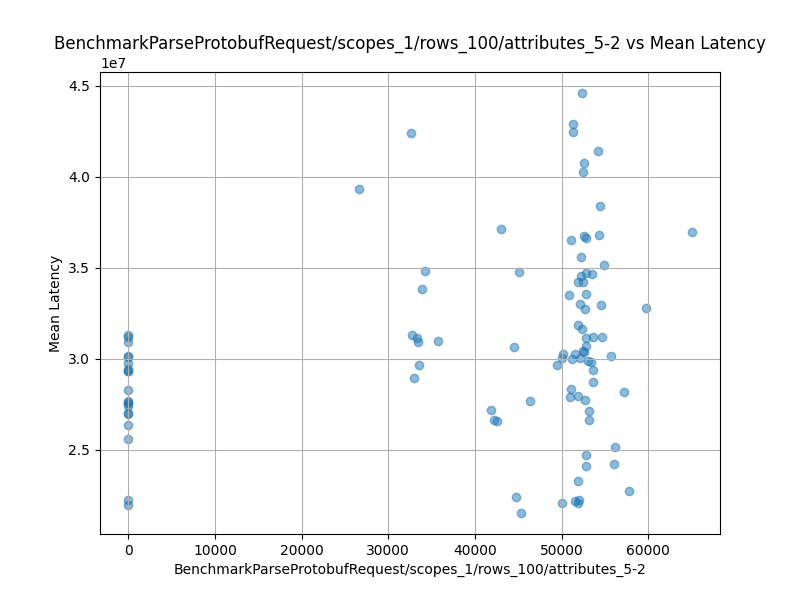
\includegraphics[width=\textwidth]{figures/BenchmarkParseProtobufRequest_scopes_1_rows_100_attributes_5-2_vs_mean_latency.png}
        \caption{BenchmarkParseProtobufRequest-scopes-1-rows-100-attributes-5-2 vs mean query rate}
        \label{fig:BenchmarkParseProtobufRequest_scopes_1_rows_100_attributes_5-2_vs_mean_latency}
    \end{subfigure}
    \hfill
     \begin{subfigure}[b]{0.45\textwidth}
        \centering
        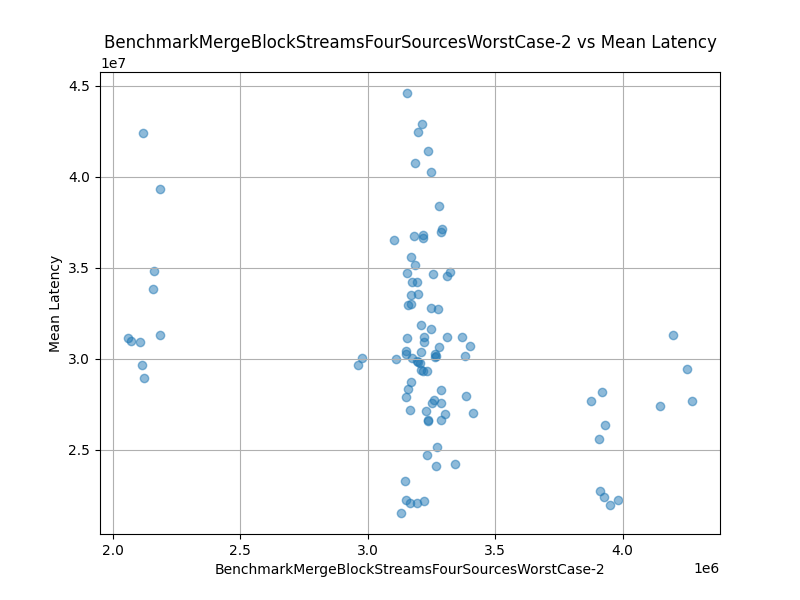
\includegraphics[width=\textwidth]{figures/BenchmarkMergeBlockStreamsFourSourcesWorstCase-2_vs_mean_latency.png}
        \caption{BenchmarkMergeBlockStreamsFourSourcesWorstCase vs mean query rate}
        \label{fig:BenchmarkMergeBlockStreamsFourSourcesWorstCase-2_vs_mean_latency}
    \end{subfigure}
    \caption{Microbenchmark vs mean rate query}
    \label{fig:micro-vs-mean-query}
\end{figure}

\cref{fig:BenchmarkQueueThroughputConcurrent_vs_mean_latency,fig:BenchmarkUnmarshalDeltaConstArray-2_vs,fig:BenchmarkParseProtobufRequest_scopes_1_rows_100_attributes_5-2_vs_mean_latency,fig:BenchmarkMergeBlockStreamsFourSourcesWorstCase-2_vs_mean_latency} confirm that the relationship between microbenchmark execution and application latency is not linear. We observe a vertical concentration of data points, indicating microbenchmark values do not correlate linearly with the mean query rate. \\
Instead, the mean query rate variates significantly for similar microbenchmark values, indicating that other factors influence performance changes beyond what our current model captures. These findings confirm that ridge regression, which assumes a linear relationship, is not well-suited for such variations, resulting in limited predictive accuracy. \\
\cref{fig:distribution_BenchmarkMergeBlockStreamsFourSourcesWorstCase-2}
portrays evidence that overfitting remains a core challenge and that increasing the number of pairs of versions does not resolve the model generalization problem. Instead, \cref{fig:DistributionMicrobenchamrk} suggests that the model memorizes behavioral patterns from the training but fails to apply them to the new data. Collinearity continues to challenge the models by adding noise to the predictions; hence, the model struggles to find an appropriate function to predict the application's performance based on microbenchmarks. \\
Even though Grambow et al. \cite{grambow} research showed that microbenchmark results could serve as a proxy for application benchmark performance (despite certain limitations), we could not replicate or refute his findings in our study, as our modeling approach did not yield robust predictions to confirm or contradict his results. These outcomes suggest that unless the effects of data distribution are carefully addressed, future research might expand on Grambow et al. \cite{grambow} research by applying more advanced statistical models or alternative regression techniques to evaluate whether microbenchmarks can reliably predict application-level performance.

\subsection{Limitations and Future Research}
\label{cha:limitationsFurtherWork}
This study provides valuable insights into comparing microbenchmark and application benchmarks. However, important limitations present in this research must be analyzed so that further research can use this work as a baseline to improve different aspects of the model’s feature selection and possibly get more accurate results. \\
When using statistical models to predict any value, the amount of data we have plays a significant role in how good the predictions might be; hence, one limitation in this study is the number of tested versions. This research conducted the experiments on a limited selection of pairs of versions, which may not fully reflect long-term performance trends or capture all possible variations across different software updates. It is probable that they do not accurately represent long-term performance trends.
Moreover, using an average-based performance metric is another limitation of this research; the detected outliers while running experiments highly influence average metrics results because they might introduce noise into the overall results, leading to inaccurate and poor performance conclusions. For this matter, future research should explore using other metrics that are not as sensitive to outliers, for instance, using median performance metrics; by implementing this metric type, further research could minimize the impact of unusual outliers in the overall performance result and obtain a more suitable model that proves a correlation between the performance change detected in a microbenchmark and its impact on the application’s benchmark performance.  \\
Additionally, the fact that this research evaluated only one system (VictoriaMetrics) is another limitation of this study. Even though relying on VictoriaMetrics allowed us to do an in-depth analysis by running the application benchmark and microbenchmark results on the same SUT, it limits the applicability of the findings to other SUTs because other optimizations might need to be done in different systems under tests which might influence the overall performance results of the application benchmark and microbenchmarks. \\
Lastly, this study uses a ridge regression model to predict if microbenchmark results predict the application benchmark performance. Even though ridge regression helps manage collinearity among features, its linear nature makes it less effective in capturing complex patterns in performance data. Therefore, we recommend that further research focus on more advanced methods to predict performance, such as decision trees or deep learning models, and see if we get reliable results. Thus, further research can use these results to investigate more about the clusters found in the distribution of the data shown in \cref{fig:distribution_BenchmarkMergeBlockStreamsFourSourcesWorstCase-2,fig:distribution_BenchmarkParseProtobufRequest_scopes_1_rows_100_attributes_5-2,fig:distribution_BenchmarkQueueThroughputConcurrent_block,fig:distribution_BenchmarkUnmarshalDeltaConstArray-2} and analyze if the clusters that present a better linear distribution would better fit a linear regression method. In addition to this, a dimensionality reduction could be applied to improve accuracy. Addressing these challenges would improve microbenchmark-based performance models' predictability and increase their ability to detect significant application benchmark performance trends. Future research can refine the benchmarking process to get more accurate results by incorporating more advanced modeling techniques, expanding dataset coverage, and validating results across multiple database systems, improving its value in assessing software performance under real-world conditions.  